% !TeX encoding = UTF-8
% !TeX spellcheck = en_GB
%%%%%%%%%%%%%%%%%%% Thesis_AndreGuerra.tex %%%%%%%%%%%%%%%%%%%%%%%%
%
% PhD Thesis - Main File
% André Guerra
%
% 04/Apr/2017
%
%%%%%%%%%%%%%%%%%%%%%%%%%%%%%%%%%%%%%%%%%%%%%%%%%%%%%%%%%%%%%%%%%%%


%------------------------------------------------------------
%% HEADER
%------------------------------------------------------------
\documentclass[a4paper, twoside, openright, 11pt, UKenglish]{book}
%draft

% -----------------------------------------------------------
% Define all configuration parameters
% -----------------------------------------------------------
% !TeX encoding = UTF-8
% !TeX spellcheck = en_GB
% !TeX root = ../ThesisTemplate_AndreGuerra.tex
%%%%%%%%%%%%%%%%%%% Thesis_AG_Preamble.tex %%%%%%%%%%%%%%%%%%
%
% PhD thesis - Preamble
% André Guerra
%
% 04/Apr/2017
%
%%%%%%%%%%%%%%%%%%%%%%%%%%%%%%%%%%%%%%%%%%%%%%%%%%%%%%%%%%%%%

%------------------------------------------------------------
%% General ------------------------------------------------%%

\pdfminorversion = 7

% Comments and review packages
\usepackage{lipsum}     % For draft text
\usepackage[linecolor=red,figcolor=white,colorinlistoftodos,%
]{todonotes}                                                % TEMP command to review
\newcommand{\review}[1]{{\textcolor{red}{\framebox{#1}}}}	% TEMP command to review

%%% Book configurations for report class
%%\makeatletter % changes the catcode of @ to 11
    %%\newcommand\frontmatter{%
        %%\cleardoublepage
        %%%\@mainmatterfalse
        %%\pagenumbering{roman}
    %%}
%%
    %%\newcommand\mainmatter{%
        %%\cleardoublepage
        %%% \@mainmattertrue
        %%\pagenumbering{arabic}
    %%}
%%
    %%\newcommand\backmatter{%
        %%\if@openright
        %%\cleardoublepage
        %%\else
        %%\clearpage
        %%\fi
        %%% \@mainmatterfalse
    %%}
%%\makeatother % changes the catcode of @ back to 12

%------------------------------------------------------------
%% Language -----------------------------------------------%%
\usepackage[main=UKenglish,portuguese]{babel}   % Language hyphenation and typographical rules
\usepackage[T1]{fontenc}                        % Use 8-bit encoding that has 256 glyphs
\usepackage[utf8]{inputenc}                     % Accept different input encodings.

\babeltags{pt = portuguese}
%\textpt{Portuguese text}
%\begin{pt}
%    Portuguese text
%\end{pt}

% For quoting phrases
\usepackage[autostyle=true,english=british]{csquotes}

%------------------------------------------------------------
%% Page geometry and others & TOC -------------------------%%
\usepackage{geometry}	
\geometry{verbose,
    a4paper,
    twoside,                        % switches on twoside mode with left and right margins swapped on verso pages
    includehead,                    % includes the head of the page
    includefoot,                    % includes the foot of the page
    textheight      = 674pt,        % the height of body (the text area)
    textwidth       = 445pt,        % the width of body (the text area)
    headheight      = 40.0pt,       % height of header
    headsep         = 21.68121pt,   % separation between header and text
    footskip        = 27.46295pt,   % distance separation between baseline of last line of text and baseline of footer
    marginparsep    = 7.0pt,        % separation between body and marginal notes
    marginparwidth  = 70pt,         % width of the marginal notes
    inner           = 22mm          % left margin (for oneside) or inner margin (for twoside)
    %
    %outer=25mm,
    %top=30mm,
    %bottom=20mm,
    %headheight=15pt
}
\marginparpush = 5.0pt

% Depth of TOC
\setcounter{secnumdepth}{3}
\setcounter{tocdepth}{2}

% Control over table of contents, figures, etc
\usepackage{tocloft}

% General purpose hierarchical index generator
\usepackage{makeidx}
\makeindex

% Nomenclature package
\usepackage[english]{nomencl}
\makenomenclature
\usepackage{ifthen}
% For multicolumn environment check ``Customisations'' bellow
% Use \vfill\null\columnbreak before ``\item[\textbf{'' to force the title to another column (in a multicolum environment)
% Use \vfill\null\clearpage in for inside a multicolum environment
\renewcommand{\nomgroup}[1]{%
    \ifthenelse{\equal{#1}{R}}{\item[\textbf{Roman Symbols}]}{%
        \ifthenelse{\equal{#1}{G}}{\item[\textbf{Greek Symbols}]}{%
            \ifthenelse{\equal{#1}{A}}{\item[\textbf{Acronyms/Abbreviations}]}{%
                \ifthenelse{\equal{#1}{T}}{\item[\textbf{Superscripts}]}{%
                    \ifthenelse{\equal{#1}{S}}{\item[\textbf{Subscripts}]}{%
                        \ifthenelse{\equal{#1}{X}}{\item[\textbf{Other Symbols}]}{%
                            \ifthenelse{\equal{#1}{E}}{\item[\textbf{Electronic Symbols}]}
                            {}
                        }% matches Electronic Roman symbols > E
                    }% matches mathematical symbols > X
                }% matches Subscripts           > T
            }% matches Superscripts         > R
        }% matches Abbreviations        > A
    }% matches Greek Symbols        > G
}% matches Roman Symbols        > R
%
%% To add some text before printing the list of symbols
\renewcommand{\nompreamble}{This is a list of several symbols and abreviations used within the body of the document. The relevant symbols' values and units are shown on the right margin.}
%
% This will add the units to the symbols
%----------------------------------------------
\newcommand{\nomunit}[1]{\renewcommand{\nomentryend}{\hspace*{\fill}#1}}
%----------------------------------------------

% Appendix
\usepackage[page,titletoc]{appendix}
\renewcommand{\appendixpagename}{Appendix}

% Include PDF documents in LaTeX
\usepackage{pdfpages}

%------------------------------------------------------------
%% Font & Paragraph ---------------------------------------%%
\usepackage{sansmathfonts}                      % For math fonts
\usepackage[scaled]{helvet}                     % Font family
\renewcommand{\familydefault}{\sfdefault}
\renewcommand{\rmdefault}{\sfdefault}

\usepackage{soul}       % For underlining

\usepackage{sectsty}    % change the style of any or all of LATEX's sectional headers
\allsectionsfont{\sfdefault}

\usepackage{fncychap}   % for changing chapter level headings
% CHAPTER font size
\ChNameVar{\fontsize{14}{16}\usefont{OT1}{phv}{m}{n}\selectfont}
\ChNumVar{\fontsize{60}{62}\usefont{OT1}{ptm}{m}{n}\selectfont}
\ChTitleVar{\Huge\bfseries\rm} \ChRuleWidth{1pt}
% Font size of number X
\ChNumVar{\raggedleft\fontsize{20pt}{25pt}\usefont{OT1}{ptm}{m}{n}\selectfont}
\ChTitleVar{\raggedright\rm\fontsize{20pt}{25pt}\bfseries\selectfont}
\ChNameAsIs
\ChNameVar{[1]}

% Chapter style
\ChNameUpperCase
\ChNameVar{\Huge\sf\bf\flushleft}
\ChNumVar{\Huge\sf\bf}
\ChTitleVar{\huge\bf\raggedright}
% Section Style
\sectionfont{\Large\raggedright}
\subsectionfont{\large\raggedright}
\subsubsectionfont{\normalsize\raggedright}

% settings for paragraphs
\setlength{\parskip}{2mm}
% defining the space between lines (1.5 is for double-space)
\usepackage{setspace}
\onehalfspacing
%%\renewcommand{\baselinestretch}{1.5}

% AMS mathematical facilities for LaTeX.
\usepackage{amsmath,amsfonts,amssymb,bm}

\usepackage{eurosym}            % Euro sign

\usepackage[per-mode = symbol,binary-units = true]{siunitx}
\sisetup{group-minimum-digits = 4}  % Group with a minimum of 4 numbers (i.e. 1 000)
\DeclareSIUnit{\EUR}{\text{\euro}}
\DeclareSIUnit[number-unit-product = {}]{\degree}{\SIUnitSymbolDegree}

\usepackage{cancel}     % To have symbols crossed on equations
\usepackage{gensymb}    % Provides generic commands (\degree, \celsius, \perthousand, \micro and \ohm)
\usepackage{xfrac}      % allows the user to typeset fractions in the form 'n/d' (\sfrac{1}{2})

% Prevent hyphenation and paragraph breaks
%\hyphenpenalty=10000
%\brokenpenalty=5000
%\clubpenalty=5000
%\widowpenalty=5000

\flushbottom    % makes all text pages the same height

\usepackage[activate={true,nocompatibility},final,tracking=true,kerning=true,spacing=true,factor=1100,stretch=10,shrink=10]{microtype}
% activate={true,nocompatibility} - activate protrusion and expansion
% final - enable microtype; use "draft" to disable
% tracking=true, kerning=true, spacing=true - activate these techniques
% factor=1100 - add 10% to the protrusion amount (default is 1000)
% stretch=10, shrink=10 - reduce stretchability/shrinkability (default is 20/20)
\microtypecontext{spacing=nonfrench}

\SetExtraKerning[unit=space]
{encoding={*}, family={*}, series={*}, size={footnotesize,small,normalsize}}
{\textendash={400,400}, % en-dash, add more space around it
    "28={ ,150}, % left bracket, add space from right
    "29={150, }, % right bracket, add space from left
    \textquotedblleft={ ,150}, % left quotation mark, space from right
    \textquotedblright={150, }} % right quotation mark, space from left

\SetExtraKerning[unit=space]
{encoding={*}, family={qhv}, series={b}, size={large,Large}}
{1={-200,-200}, 
    \textendash={400,400}}
%%
%%\SetTracking{encoding={*}, shape=sc}{40}

\usepackage{enumitem}   % Customized lists
\setlist{noitemsep}     % Make itemize lists more compact

% Numbering of equations, figures and tables
\numberwithin{equation}{chapter}
\numberwithin{figure}{chapter}
\numberwithin{table}{chapter}

\usepackage[explicit]{titlesec}
\titleformat{name=\paragraph,numberless}[runin]{\normalfont\normalsize\bfseries}{}{15pt}{#1.}

%------------------------------------------------------------
%% Graphics & Figures -------------------------------------%%
\usepackage{xcolor}         % Package to define colours
\definecolor{FCUPBlue}{RGB}{147,191,235}    % FCUP color

\usepackage{graphicx}   % Enhanced support for graphics.

% Custom captions under/above floats in tables or figures
\usepackage{caption}
\usepackage{subcaption}
\renewcommand{\figurename}{Fig.} %to support older versions of captions.sty
\captionsetup{format=plain,indention=0.5cm,labelsep=endash,justification=centerlast,font=footnotesize,labelfont=bf,textfont=it,tableposition=top}

\usepackage[section]{placeins}  % ensure all floats for a section appear before the next \section command
\usepackage{flafter}            % force floats to appear after they are defined

\usepackage{epstopdf}   % To include eps figures

\usepackage{booktabs}   % For professional looking tables
\usepackage{multirow}   % Create tabular cells spanning multiple rows
\usepackage{multicol}   % Create tabular cells spanning multiple columns
\usepackage{rotating}   % To rotate tables and cell text
\usepackage{threeparttable} % tables with footnotes

% To use pgf-tikz figures
\usepackage{pgf,tikz}
\usepackage{mathrsfs}
\usetikzlibrary{arrows}
\usetikzlibrary[patterns]
\usepackage{pgfplots}
\pgfplotsset{compat=1.15}

% Path to the figures directory
\graphicspath{
    {1_Figs/}
    {01_FrontMatter/Figs/}
    {10_Introduction/Figs/}
    {20_SmallSatellites/Figs/}
    {30_Oceanography/Figs/}
    {40_IntegratedScenario/Figs/}
    {50_ThermalAnalysis/Figs/}
    {80_Appendices/Figs/}}

%------------------------------------------------------------
%% Links and Bookmarks ------------------------------------%%
\RequirePackage[hyphens]{url}   % To include urls on document and bibliography

% 'hyperref' package
\RequirePackage{hyperref} % enhance documents that are to be output as HTML and PDF
\hypersetup{
    colorlinks          = true,         % color text of links and anchors, eliminates borders around links
    allcolors           = black,        % color for anchor text (black)
    bookmarksnumbered   = true,         % put section numbers in bookmarks
    breaklinks          = true,         % allow links to break over lines 
    %citecolor           = FCUPblue,     % color of citation links
    %backref             = true,         % do bibliographical back references
    %
    pdfdisplaydoctitle  = true,         % display document title instead of file name in title bar
    pdfpagelayout       = OneColumn,    % set layout of PDF pages
    pdfstartview        = FitH,         % starting view of PDF document
    pdfpagemode         = UseNone,      % set default mode of PDF display (UseOutlines)
    %
    pdftitle            = {PhD Thesis Andre Guerra},
    pdfauthor           = {Andre Guerra},
    pdfsubject          = {PhD thesis of Andre Guerra.}%,
    %pdfkeywords         = {\@keywords}    
}

\usepackage[figure,table]{hypcap}       % Adjusting the anchors of captions.

\usepackage[open,openlevel=0]{bookmark} % For advanced bookmark options

%------------------------------------------------------------
%% Bibliography -------------------------------------------%%
\usepackage[square,comma,numbers,sort&compress,longnamesfirst]{natbib}

\usepackage{notoccite}  % Prevent trouble from citations in table of contents, etc

\usepackage{doi}        % hyperlink DOI numbers to dx.doi.org

%------------------------------------------------------------
%% Headers and Footers ------------------------------------%%
\usepackage{fancyhdr}

\pagestyle{fancy}   % Defines the page style to fancy
\fancyhf{}          % Clear headers and footers

%%%% Headers
% Remove headers and footers on blank pages
\makeatletter % changes the catcode of @ to 11
\def\cleardoublepage{\clearpage\if@twoside \ifodd\c@page\else
    \hbox{}
    %\vspace*{\fill}
    %\begin{center}
    %This page intentionally contains only this sentence.
    %\end{center}
    %\vspace{\fill}
    \thispagestyle{empty}
    \newpage
    \if@twocolumn\hbox{}\newpage\fi\fi\fi}
\makeatother % changes the catcode of @ back to 12

% Define chapter name in smallcaps at header
\renewcommand{\chaptermark}[1]{\markboth{#1}{a}}     
\renewcommand{\sectionmark}[1]{\markright{\thesection\ #1}}

% Remove header and footer lines
\renewcommand{\headrulewidth}{0pt}
\renewcommand{\footrulewidth}{0pt}

%%%% Change chapter top margin
\makeatletter % changes the catcode of @ to 11
% For the case \chapter
\renewcommand*{\@makechapterhead}[1]{%
    \vspace*{1\p@}%
    {\parindent \z@ \raggedright \normalfont
        \ifnum \c@secnumdepth >\m@ne
        \if@mainmatter    % Fix for frontmatter, mainmatter, and backmatter 040920
        \DOCH
        \fi
        \fi
        \interlinepenalty\@M
        \if@mainmatter  % Fix for frontmatter, mainmatter, and backmatter 060424
        \DOTI{#1}%
        \else%
        \DOTIS{#1}%
        \fi
}}
% For the case \chapter*
\renewcommand*{\@makeschapterhead}[1]{%
    \vspace*{1\p@}%
    {\parindent \z@ \raggedright
        \normalfont
        \interlinepenalty\@M
        \DOTIS{#1}
        \vskip 10\p@
}}
\makeatother % changes the catcode of @ back to 12

\fancypagestyle{myfancy}{
    % Odd pages with right side header
    \fancyhead[RO]{
        \begin{tabular}{r|c} %%% REMOVE (\textbf{DRAFT \today}) for final version!!!
            {\fontsize{8pt}{8pt}\selectfont FCUP (\textbf{DRAFT \today})}                   & \multirow{2}{*}{\fontsize{8pt}{10pt}\selectfont\thepage} \\
            {\fontsize{8pt}{8pt}\selectfont\nouppercase\rightmark}  & \\
        \end{tabular}%
    }
    %
    % Even pages with left side header
    \fancyhead[LE]{
        \begin{tabular}{c|l} %%% REMOVE (\textbf{DRAFT \today}) for final version!!!
            \multirow{2}{*}{\fontsize{8pt}{10pt}\selectfont \thepage}           & {\fontsize{8pt}{8pt}\selectfont FCUP (\textbf{DRAFT \today})} \\
            & {\fontsize{8pt}{8pt}\selectfont\nouppercase\leftmark} \\
        \end{tabular}%
    }
    %
    % Odd (Even) pages left (right) side header
    \fancyhead[LO,RE]{
        \raisebox{-0.4\height}{
\includegraphics[height=30pt, keepaspectratio=true]{FCUP_eps}}
    }
}

\fancypagestyle{plain}{%
    \fancyhead[RO,LE]{{\fontsize{8pt}{10pt}\selectfont\thepage}}
    \fancyhead[LO,RE,CE,CO]{}
}
\fancypagestyle{myfrontmatter}{%
    \fancyhead[RO,LE]{{\fontsize{8pt}{10pt}\selectfont\thepage}}
    \fancyhead[LO,RE,CE,CO]{}
}

% Footnotes
\usepackage{footnote}
% Footnote style
\renewcommand{\thefootnote}{\roman{footnote}}
\interfootnotelinepenalty=10000

%------------------------------------------------------------
%% Customisations -----------------------------------------%%

% Change the way nomenclature is presented
\makeatletter % changes the catcode of @ to 11
    \@ifundefined{chapter}
    {\def\wilh@nomsection{section}}
    {\def\wilh@nomsection{chapter}}
    
    \def\thenomenclature{%
        \begin{multicols*}{2}[%
            \csname\wilh@nomsection\endcsname*{\nomname}
            \if@intoc\addcontentsline{toc}{\wilh@nomsection}{\nomname}\fi
            \nompreamble]
            \setlength{\columnsep}{1cm}
            \setlength{\columnseprule}{1pt}
            \list{}{%
                \labelwidth\nom@tempdim
                \leftmargin\labelwidth
                \advance\leftmargin\labelsep
                \itemsep\nomitemsep
                \let\makelabel\nomlabel
            }%
        }
        
        \def\endthenomenclature{%
            \endlist
        \end{multicols*}
   \nompostamble}
\makeatother % changes the catcode of @ back to 12

%------------------------------------------------------------
%% Standarisation -----------------------------------------%%

% Hyperref package names for referecing parts of text
% Macro                 Default
%\figurename            Figure          % Reference a figure
%\tablename             Table           % Reference a table
%\appendixname          Appendix
%\equationname          Equation
%\chaptername           chapter
%\sectionname           section         % Reference a section
%\subsectionname        subsection
%\subsubsectionname     subsubsection
%\paragraphname         paragraph
%\Hfootnotename         footnote

\addto\extrasUKenglish{%
    \renewcommand{\chapterautorefname}{Chapter}%
}
\addto\extrasUKenglish{%
    \renewcommand{\sectionautorefname}{Section}%
}
\addto\extrasUKenglish{%
    \renewcommand{\subsectionautorefname}{Section}%
}
\addto\extrasUKenglish{%
    \def\equationautorefname~#1\null{Equation~(#1)\null}%
}


% end of file Thesis_AG_Preamble.tex
%%%%%%%%%%%%%%%%%%%%%%%%%%%%%%%%%%%%%%%%%%%%%%%%%%%%%%%%%%%%%%%%%%% % file "Thesis_Preamble.tex"


%------------------------------------------------------------
%% DOCUMENT
%------------------------------------------------------------
\begin{document}

%------------------------------------------------------------
%% Title Page ---------------------------------------------%%

\makeatletter % changes the catcode of @ to 11
    \title{Small Satellites and Oceanography XX}    \let\Title\@title
    \author{\textpt{Andr\'e Gomes da Costa Guerra}} \let\Author\@author
    \date{\the\year}                                \let\Date\@date
\makeatother % changes the catcode of @ back to 12



%------------------------------------------------------------
%% Front matter -------------------------------------------%%
\frontmatter
\pagestyle{plain}

%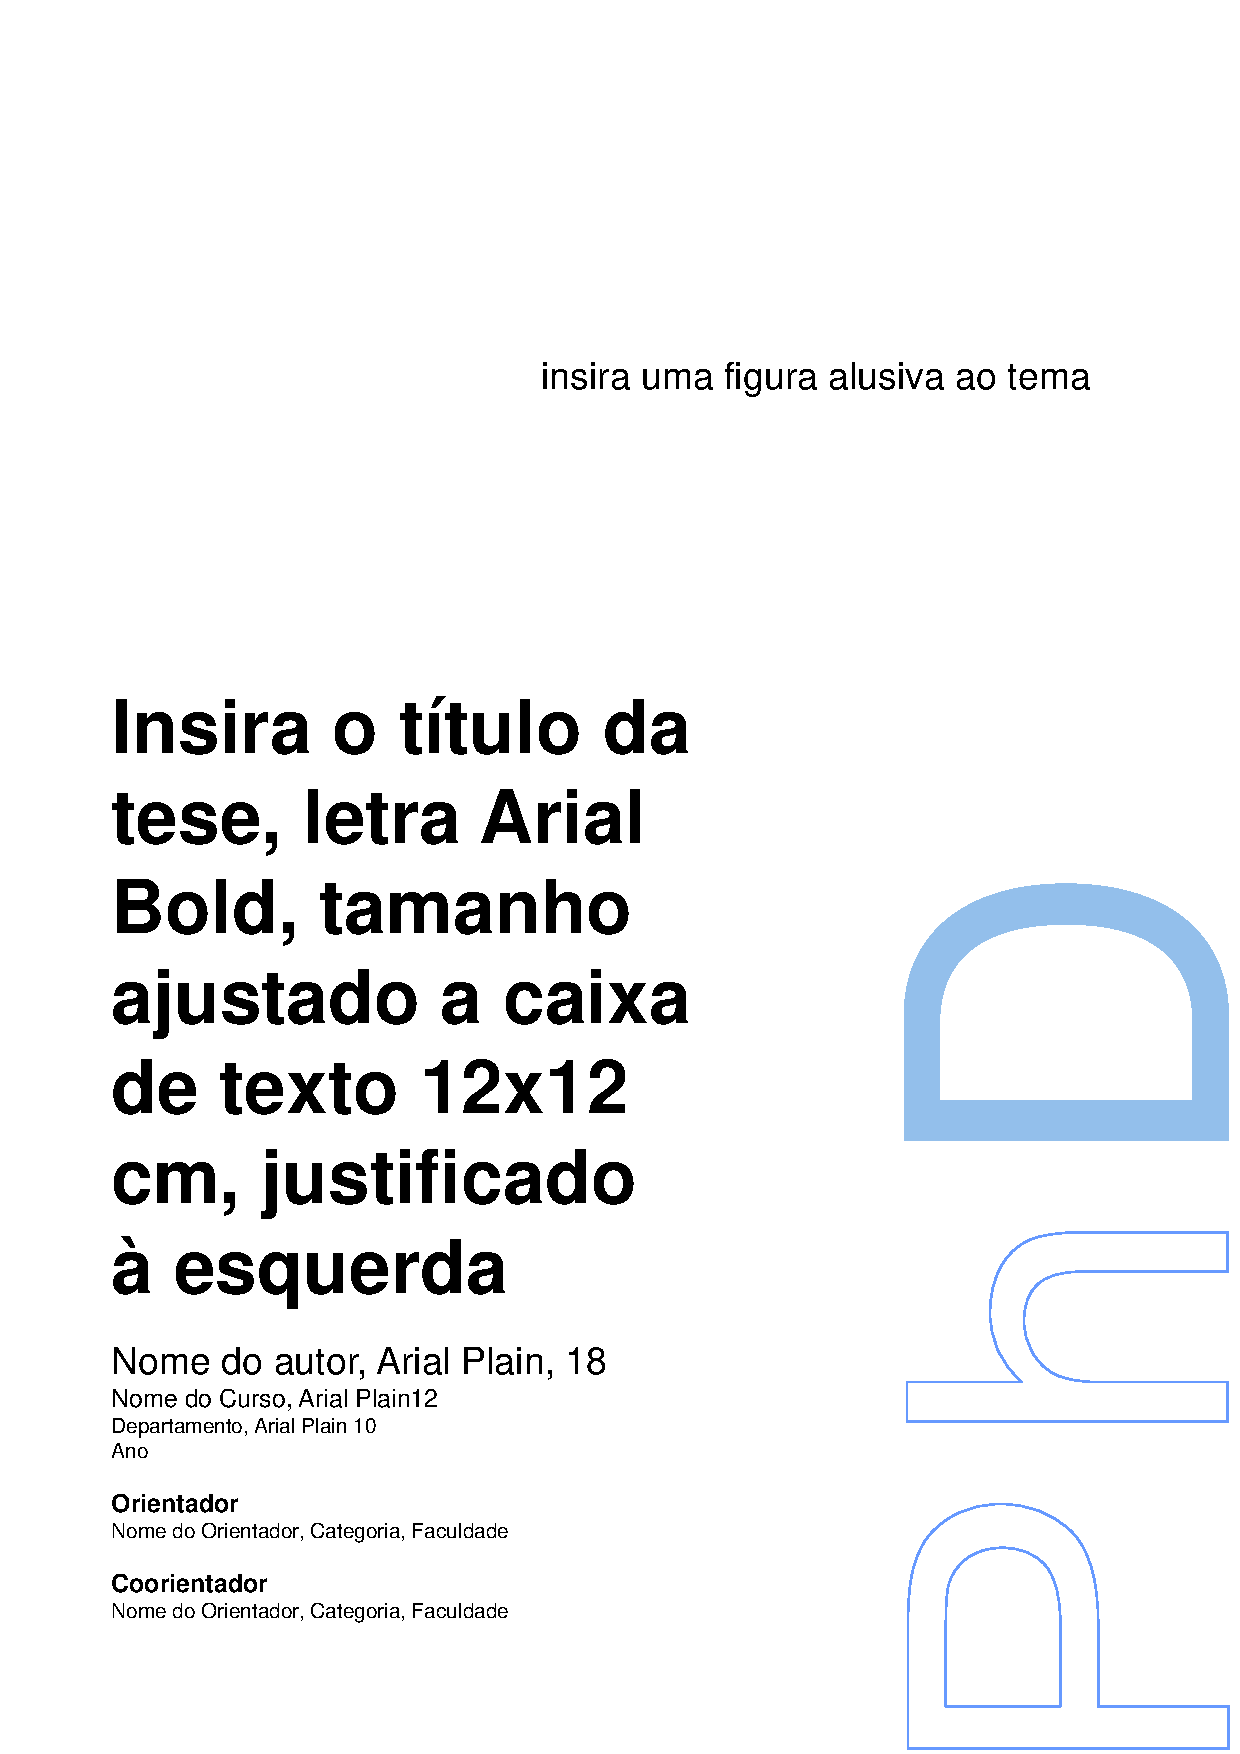
\includepdf{01_FrontMatter/FolhaRostoMAP_v0}
%\cleardoublepage

% !TeX encoding = UTF-8
% !TeX spellcheck = en_GB
% !TeX root = ../ThesisTemplate_AndreGuerra.tex
%%%%%%%%%%%%%%%%%%%% Thesis_Titlepage.tex %%%%%%%%%%%%%%%%%%%
%
% PhD thesis - Title Page
% André Guerra
%
% 18/Apr/2017
%
%%%%%%%%%%%%%%%%%%%%%%%%%%%%%%%%%%%%%%%%%%%%%%%%%%%%%%%%%%%%%


\newpage{
    \thispagestyle{empty}
    
    \null\vskip 2cm%
    
    %
    % Author and Title
    \begin{center}
        {\LARGE \bf \Author}            \\
        \vskip 1.5cm
        %
        \begin{doublespace}
            {\Huge \bf \expandafter{\Title}}
        \end{doublespace}
    \end{center}

    \vskip 2cm%
    
    %
    % Logo
    \capstartfalse
    \begin{figure}[h!]
        \centering
        
\includegraphics[width=8cm]{FCUP_eps}
    \end{figure}
    \vfill
    
    %
    % Supervisor
    \begin{center}
        {\normalsize \it \textbf{Supervisor:} Professor Orfeu Bertolami Neto}    \\
    \end{center}
    \vfill
    
    %
    % MAP-fis text
    \begin{center}
        {\small \it Thesis submitted to the Faculty of Sciences of the University of Porto      \\
        in partial fulfilment of the requirements for the degree of Doctor in Physics}          \\
    \end{center}
    \vfill
    
    %
    % Department
    \begin{center}
        \expandafter{
            Centro de F\'{i}sica do Porto                   \\
            Department of Physics and Astronomy             \\
            Faculty of Sciences of the University of Porto} \\
        \vskip 0.3cm%
        \Date \\
    \end{center}
    \vskip 1cm
}

\newpage{
    \thispagestyle{empty}
    
    \null\vfill
    
    %
    % Copyrights
    \begin{center}
        \footnotesize
        \textcopyright\ \Date \\
        \Author \\
        ALL RIGHTS RESERVED \\
    \end{center}
}

% end of file Thesis_Titlepage.tex
%%%%%%%%%%%%%%%%%%%%%%%%%%%%%%%%%%%%%%%%%%%%%%%%%%%%%%%%%%%%%%%%%%%
%\cleardoublepage

% !TeX encoding = UTF-8
% !TeX spellcheck = en_GB
% !TeX root = ../Thesis_AndreGuerra.tex
%%%%%%%%%%%%%%% Thesis_InstitutionsFunding.tex %%%%%%%%%%%%%%
%
% PhD thesis - Institutions Involved and Funding
% André Guerra
%
% 18/Apr/2017
%
%%%%%%%%%%%%%%%%%%%%%%%%%%%%%%%%%%%%%%%%%%%%%%%%%%%%%%%%%%%%%


\newpage{
    \thispagestyle{empty}
    
    \Large{Institutions where the work was carried out:}
    
    \vskip 1cm
    
    \capstartfalse
    \begin{figure}[h!]
        \centering
        \begin{subfigure}[c]{0.45\textwidth}
            \centering
            
\includegraphics[width=0.9\textwidth]{FCUP_eps}
        \end{subfigure}
        \hfill %add desired spacing between images, e. g. ~, \quad, \qquad, \hfill etc. 
          %(or a blank line to force the subfigure onto a new line)
        \begin{subfigure}[c]{0.45\textwidth}
            \centering
            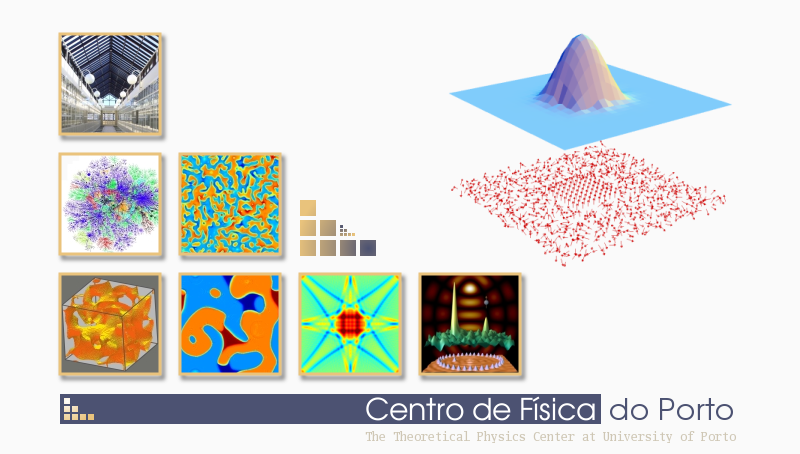
\includegraphics[width=0.7\textwidth]{CFP}
        \end{subfigure}
        
        \vspace*{0.4cm}
        
        \begin{subfigure}[c]{0.45\textwidth}
            \centering
            
\includegraphics[width=0.4\textwidth]{LSTS}
        \end{subfigure}
        \hfill %add desired spacing between images, e. g. ~, \quad, \qquad, \hfill etc. 
          %(or a blank line to force the subfigure onto a new line)
        \begin{subfigure}[c]{0.45\textwidth}
            \centering
            
\includegraphics[width=0.8\textwidth]{UVigo}
        \end{subfigure}
    \end{figure}
    
    \vskip 2cm

    \Large{Funding:}
    
    My PhD work was supported by the Funda{\c c}\~ao para a Ci\^encia e a Tecnologia (Portuguese Agency for Research) fellowship PD/BD/XXXXXX/XXXX.
    
    \vskip 1cm
    
    \begin{figure}[h!]
        \centering
        
\includegraphics[width=0.5\linewidth]{FCT}
        \caption*{}
    \end{figure}
    
    \vfill
}

% end of file Thesis_InstitutionsFunding.tex
%%%%%%%%%%%%%%%%%%%%%%%%%%%%%%%%%%%%%%%%%%%%%%%%%%%%%%%%%%%%%%%%%%%
\cleardoublepage

% !TeX encoding = UTF-8
% !TeX spellcheck = en_GB
% !TeX root = ../ThesisTemplate_AndreGuerra.tex
%%%%%%%%%%%%%%%%% Thesis_DedicationQuote.tex %%%%%%%%%%%%%%%%
%
% PhD thesis - Dedication or Quote
% André Guerra
%
% 18/Apr/2017
%
%%%%%%%%%%%%%%%%%%%%%%%%%%%%%%%%%%%%%%%%%%%%%%%%%%%%%%%%%%%%%

% Dedication
\newpage{
    \thispagestyle{empty}
    
    \vspace*{2cm} % Change value to choose place
    
    \capstartfalse
    \begin{table}[!tbh]  
        \hspace*{10cm}  % Change value to choose place
        \raggedright
        \begin{tabular}{ l }
            \textit{To my grandmother,}\\
            \textit{my parents,}\\
            \textit{my brother}\\
            \textit{and Carolina.}\\
        \end{tabular}
    \end{table}
}

% Or Quote !!!
%%\newpage{
    %%\thispagestyle{empty}
    %%\null\vskip 0.2in
    %%\vfill
    %%\vfill
    %%
    %%\vskip .8in
    %%
    %%\large \bf \expandafter{
    %%
    %%\begin{table}[!ht]
        %%\begin{minipage}[b]{0.17\linewidth}
            %%%\vspace{-20pt}
            %%%\includegraphics[scale=0.65]{./FIGBOOK1/P4/P14_FIG02}
            %%%\vspace{-20pt}
        %%\end{minipage}
        %%
        %%\hspace{0.20\linewidth}
        %%
        %%\begin{minipage}[b]{0.75\textwidth}
            %%%\raggedright
            %%\begin{quote}
            %%{\fontsize{9pt}{16pt}\selectfont 
            %%\textit{``The Wheel of Time turns, and Ages come and pass, leaving memories that become legend. Legend fades to myth, and even myth is long forgotten when the Age that gave it birth comes again. In one Age, called the Modern Age by some, an Age yet to come, an Age long past, a wind rose in the Mountains of Mist. The wind was not the beginning. There are neither beginnings nor endings to the turning of the Wheel of Time. But it was a beginning.''}}
            %%\end{quote}
            %%\center
            %%\textit{\textbf{Robert Jordan},\\ \textit{``The Wheel of Time Series''}}
        %%\end{minipage}
    %%\end{table}
    %%}
%%}



% end of file Thesis_DedicationQuote.tex
%%%%%%%%%%%%%%%%%%%%%%%%%%%%%%%%%%%%%%%%%%%%%%%%%%%%%%%%%%%%%%%%%%%
\cleardoublepage

% !TeX encoding = UTF-8
% !TeX spellcheck = en_GB
% !TeX root = ../Thesis_AndreGuerra.tex
%%%%%%%%%%%%%%%%%%% Thesis_Preface.tex %%%%%%%%%%%%%%%%%%%%%%%%%%%%%%%%%%
%
% PhD Thesis - Preface
% André Guerra
%
% 09/Jan/2018
%
%%%%%%%%%%%%%%%%%%%%%%%%%%%%%%%%%%%%%%%%%%%%%%%%%%%%%%%%%%%%%%%%%%%


% ---------------------------------------------
% ---------------------------------------------
\chapter*{Preface}
\label{chp:Preface}
\addcontentsline{toc}{chapter}{Preface}

\textbf{This part is just a summary of the work developed, why was it like that, what was accomplished, the papers published and so on.}

{\small\textit{\lipsum[1-2]}}


% end of file Thesis_Preface.tex
%%%%%%%%%%%%%%%%%%%%%%%%%%%%%%%%%%%%%%%%%%%%%%%%%%%%%%%%%%%%%%%%%%%
\cleardoublepage

% !TeX encoding = UTF-8
% !TeX spellcheck = en_GB
% !TeX root = ../Thesis_AndreGuerra.tex
%%%%%%%%%%%%%%%% Thesis_Acknowledgements.tex %%%%%%%%%%%%%%%%
%
% PhD thesis - Acknowledgements
% André Guerra
%
% 04/Apr/2017
%
%%%%%%%%%%%%%%%%%%%%%%%%%%%%%%%%%%%%%%%%%%%%%%%%%%%%%%%%%%%%%

\markboth{Acknowledgements}{Acknowledgements}
\chapter*{Acknowledgements}
%\addcontentsline{toc}{chapter}{Acknowledgements}

\lipsum[3-6]

\vspace{10mm}
{\flushleft{The author name}}

% end of file Thesis_Acknowledgements.tex
%%%%%%%%%%%%%%%%%%%%%%%%%%%%%%%%%%%%%%%%%%%%%%%%%%%%%%%%%%%%%%%%%%%
\cleardoublepage

% !TeX encoding = UTF-8
% !TeX spellcheck = en_GB
% !TeX root = ../Thesis_AndreGuerra.tex
%%%%%%%%%%%%%%%%%%%% Thesis_Abstract.tex %%%%%%%%%%%%%%%%%%%%
%
% PhD thesis - Resumo & Abstract
% André Guerra
%
% 04/Apr/2017
%
%%%%%%%%%%%%%%%%%%%%%%%%%%%%%%%%%%%%%%%%%%%%%%%%%%%%%%%%%%%%%

\hypertarget{Resumo}{}
\bookmark[level=chapter,dest=Resumo]{Resumo}
\markboth{Resumo}{Resumo}
\chapter*{Resumo}
%\addcontentsline{toc}{chapter}{Resumo}

\begin{pt}

{\small\textit{\lipsum[1-2]}}

\vfill

\textbf{Palavras-chave:} ...
\end{pt}

%------------------------------------------------------------
\cleardoublepage

\hypertarget{Abstract}{}
\bookmark[level=chapter,dest=Abstract]{Abstract}
\markboth{Abstract}{Abstract}
\chapter*{Abstract}
%\addcontentsline{toc}{chapter}{Abstract}

{\small\textit{\lipsum[1-2]}}

\vfill

\textbf{Keywords:} ...

% end of file Thesis_Abstract.tex
%%%%%%%%%%%%%%%%%%%%%%%%%%%%%%%%%%%%%%%%%%%%%%%%%%%%%%%%%%%%%%%%%%%
\cleardoublepage

%------------------------------------------------------------
%% Tables of contents -------------------------------------%%
\microtypesetup{protrusion=false} % disables protrusion locally in the document

\renewcommand{\contentsname}{Contents}
\hypertarget{Contents}{}
\bookmark[level=chapter,dest=Contents]{Contents}
\tableofcontents    % Table of contents
%\addcontentsline{toc}{chapter}{Contents}
\cleardoublepage

\renewcommand\listfigurename{List of Figures}
\hypertarget{ListofFigures}{}
\bookmark[level=chapter,dest=ListofFigures]{List of Figures}
\listoffigures      % List of Figures
%\addcontentsline{toc}{chapter}{List of Figures}
\cleardoublepage

\renewcommand\listtablename{List of Tables}
\hypertarget{ListofTables}{}
\bookmark[level=chapter,dest=ListofTables]{List of Tables}
\listoftables       % List of Tables
%\addcontentsline{toc}{chapter}{List of Tables}
\cleardoublepage

% !TeX encoding = UTF-8
% !TeX spellcheck = en_GB
% !TeX root = ../ThesisTemplate_AndreGuerra.tex
%%%%%%%%%%%%%%%%%%% Thesis_Nomenclature.tex %%%%%%%%%%%%%%%%%
%
% PhD thesis - Nomenclature
% André Guerra
%
% 04/Apr/2017
%
%%%%%%%%%%%%%%%%%%%%%%%%%%%%%%%%%%%%%%%%%%%%%%%%%%%%%%%%%%%%%

% ----------------------------------------------------------------------
% ----------------------------------------------------------------------
% Roman symbols [R]
%%\nomenclature[Ru]{$\bf u$}{Velocity vector.}
%%\nomenclature[Ru]{$u,v,w$}{Velocity Cartesian components.}
%%\nomenclature[Rp]{$p$}{Pressure.}
%%\nomenclature[RC]{$C_D$}{Coefficient of drag.}
%%\nomenclature[RC]{$C_L$}{Coefficient of lift.}
%%\nomenclature[RC]{$C_M$}{Coefficient of moment.}

% ----------------------------------------------------------------------
% ----------------------------------------------------------------------
% Greek symbols [G]
%%\nomenclature[G]{$\rho$}{Density.}
%%\nomenclature[G]{$\alpha$}{Angle of attack.}
%%\nomenclature[G]{$\beta$}{Angle of side-slip.}
%%\nomenclature[G]{$\mu$}{Molecular viscosity coefficient.}
%%\nomenclature[G]{$\kappa$}{Thermal conductivity coefficient.}

% ----------------------------------------------------------------------
% ----------------------------------------------------------------------
% Subscripts [S]
%%\nomenclature[S]{$x,y,z$}{Cartesian components.}
%%\nomenclature[S]{$i,j,k$}{Computational indexes.}
%%\nomenclature[S]{$\infty$}{Free-stream condition.}
%%\nomenclature[S]{ref}{Reference condition.}
%%\nomenclature[S]{$n$}{Normal component.}

% ----------------------------------------------------------------------
% ----------------------------------------------------------------------
% Supercripts [T]
%%\nomenclature[T]{T}{Transpose.}
%%\nomenclature[T]{*}{Adjoint.}

% ----------------------------------------------------------------------
% ----------------------------------------------------------------------
% Abbreviations [A]
% General
\nomenclature[A]{ESA}{European Space Agency.}
\nomenclature[A]{NASA}{National Aeronautics and Space Administration.}
\nomenclature[A]{FCUP}{Faculdade de Ci\^{e}ncias da Universidade do Porto.}
\nomenclature[A]{FEUP}{Faculdade de Engenharia da Universidade do Porto.}
\nomenclature[A]{UVigo}{Universidade de Vigo.}
\nomenclature[A]{LSTS}{Laboratório de Sistemas e Tecnologia Subaquática.}
\nomenclature[A]{EMEPC}{Estrutura de Missão para a Extensão da Plataforma Continental.}


% --------------------
% Small Satellites
\nomenclature[A]{LEO}{Low Earth orbit.}
\nomenclature[A]{GSO}{Geosynchronous orbit.}
\nomenclature[A]{IAA}{International Academy of Astronautics.}

\nomenclature[A]{PCB}{Printed circuit board.}

\nomenclature[A]{ADCS}{Attitude Determination \& Control System.}
\nomenclature[A]{EPS}{Electric Power System.}
\nomenclature[A]{C\&DH}{Command \& Data Handling.}
\nomenclature[A]{Comm}{Communication.}
\nomenclature[A]{GNSS}{Global Navigation Satellite System.}
\nomenclature[A]{RTG}{Radioisotope Thermoelectric Generators.}
\nomenclature[A]{COTS}{Commercial off-the-shelf.}
\nomenclature[A]{SDR}{Software defined radio.}

\nomenclature[A]{P-POD}{Poly Picosatellite Orbital Deployer.}

% Incluir estes???
\nomenclature[A]{UHF}{Ultra-high frequency.}
\nomenclature[A]{VHF}{Very high frequency.}
\nomenclature[A]{FPGA}{Field-programmable gate array.}
\nomenclature[A]{ARM}{Advanced RISC Machine}
\nomenclature[A]{MEMS}{Micro-Electro-Mechanical Systems.}
\nomenclature[A]{ITU}{International Telecommunication Union.}
\nomenclature[A]{UN}{United Nations.}
\nomenclature[A]{UNOOSA}{UN Office for Outer Space Affairs.}
\nomenclature[A]{R\&D}{Research and development.}


% --------------------
% Oceanography
\nomenclature[A]{SAR}{Synthetic Aperture Radar.}
\nomenclature[A]{LIDAR}{Light Detection and Ranging.}
\nomenclature[A]{AIS}{Automatic Identification System.}
\nomenclature[A]{GNSS-R}{Global Navigation Satellite Systems Reflectometry.}

\nomenclature[A]{DORIS}{Doppler Orbitography and Radiopositioning Integrated by Satellite.}
\nomenclature[A]{LRA}{Laser Retroreflector Array.}

\nomenclature[A]{SST}{Sea suface temperature.}

\nomenclature[A]{MDA}{Maritime Domain Awareness.}
\nomenclature[A]{ISR}{Intelligence, Surveillance, and Reconnaissance.}

\nomenclature[A]{ISS}{International Space Station.}
\nomenclature[A]{NOAA}{National Oceanographic and Atmospheric Administration.}
\nomenclature[A]{ISRO}{Indian Space Research Organization.}
\nomenclature[A]{CEOS}{Committee on Earth Observation Satellites.}
\nomenclature[A]{DND}{Canadian Department of National Defence.}
\nomenclature[A]{LAPAN}{Indonesian space agency.}
\nomenclature[A]{DLR}{German Aerospace Center.}
\nomenclature[A]{JAXA}{Japanese Aerospace Exploration Agency.}

\nomenclature[A]{CCD}{Charge-coupled device.}
\nomenclature[A]{FOV}{Field of view.}
\nomenclature[A]{VIS}{Visible spectrum.}
\nomenclature[A]{NIR}{Near infrared spectrum.}


% --------------------
% Communication
\nomenclature[A]{GEO}{Geostationary Earth orbit.}
\nomenclature[A]{IMO}{International Maritime Organisation.}

\nomenclature[A]{LGS}{Local ground station.}
\nomenclature[A]{RGS}{Remote ground station.}
\nomenclature[A]{MCC}{Mission control centre}


% --------------------
% Autonomous Vehicles
\nomenclature[A]{AUV}{Autonomous underwater vehicles.}
\nomenclature[A]{ASV}{Autonomous surface vehicles.}
\nomenclature[A]{UAV}{Unmanned aerial vehicles.}

\nomenclature[A]{GSM}{Global System for Mobile Communications.}
\nomenclature[A]{DTN}{Disruptive Tolerant Networking.}

\nomenclature[A]{EPO}{Expanded PolyOlefin foam.}

\nomenclature[A]{IMC}{Inter-Module Communication.}
\nomenclature[A]{DUNE}{Unified Navigational Environment.}


% --------------------
% HumSat System
\nomenclature[A]{RF}{Radio frequency.}
\nomenclature[A]{UART}{Universal Asynchronous Receiver-Transmitter.}
\nomenclature[A]{GMSK}{Gaussian Minimum Shift Keying modulation.}
\nomenclature[A]{CPU}{Central processing unit.}
\nomenclature[A]{TTL}{Transistor–Transistor Logic.}
\nomenclature[A]{HITL}{Hardware-in-the-Loop.}
\nomenclature[A]{DPC}{Deferred Procedure Call.}

\nomenclature[EV]{VIN}{Voltage in power pin.}
\nomenclature[EG]{GND}{Ground power pin.}
\nomenclature[ED]{DOUT}{Digital transmit pin.}
\nomenclature[ED]{DIN}{Digital receive pin.}
\nomenclature[ET]{TX}{Transmit.}
\nomenclature[ER]{RX}{Receive.}
\nomenclature[EI]{IOREF}{Input/Output reference pin.}

\nomenclature[EM]{$\mathbf{M}$}{Thermal moment.\nomunit{\si{N.m}}}

\nomenclature[EAU]{\si{AU}}{Astronomical units.\nomunit{\SI{149.6e9}{m}}}


% --------------------
% New Horizons
\nomenclature[A]{PPN}{Parameterized post-Newtonian formalism.}


% --------------------
% Appendix (SHOULD BE USED?)
\nomenclature[G]{$\theta$}{Radar antenna incident angle.}
\nomenclature[G]{$\tau$}{Radar pulse time length.}
\nomenclature[G]{$\delta_\mathrm{R}$}{Radar range resolution.}
\nomenclature[G]{$\delta_\mathrm{A}$}{Radar azimuth resolution.}
\nomenclature[G]{$\lambda$}{Radar pulse wavelength.}

\nomenclature[RS]{$S$}{Swath width.}
\nomenclature[RD]{$D$}{Length of the antenna in the spacecraft motion direction.}
\nomenclature[Rd]{$d$}{Length of the antenna perpendicular to the spacecraft motion direction.}
\nomenclature[RR]{$R$}{Distance to the centre of the swath area.}
\nomenclature[RRi]{$R_i$}{Range distance to point $i$ in the swath area.}
\nomenclature[Rc]{$c$}{Speed of light.\nomunit{\SI{299.8e6}{m/s}}}
\nomenclature[Rh]{$h$}{Spacecraft orbit altitude.}
\nomenclature[RB]{$B$}{Radar pulse bandwidth.}

\nomenclature[A]{SNR}{Radar signal-to-noise ratio.}



% end of file Thesis_Nomenclature.tex
%%%%%%%%%%%%%%%%%%%%%%%%%%%%%%%%%%%%%%%%%%%%%%%%%%%%%%%%%%%%%%%%%%%
%\begin{multicols}{2}
\begin{small}
    \markboth{Nomenclature}{Nomenclature}
    \hypertarget{Nomenclature}{}
    \bookmark[level=chapter,dest=Nomenclature]{Nomenclature}
    \printnomenclature
    %\end{multicols}
\end{small}
\cleardoublepage

\microtypesetup{protrusion=true} % enables protrusion

%------------------------------------------------------------
%% Chapters -----------------------------------------------%%
\mainmatter
\pagestyle{myfancy}

%------------------------------------------------------------
% !TeX encoding = UTF-8
% !TeX spellcheck = en_GB
% !TeX root = ../ThesisTemplate_AndreGuerra.tex
%%%%%%%%%%%%%%%%%%% 10_Intro.tex %%%%%%%%%%%%%%%%%%%%%%%%%%%%%%%%%%
%
% PhD Thesis - Introduction
% André Guerra
%
% 12/Dec/2017
%
%%%%%%%%%%%%%%%%%%%%%%%%%%%%%%%%%%%%%%%%%%%%%%%%%%%%%%%%%%%%%%%%%%%


% ---------------------------------------------
% ---------------------------------------------
\chapter{Introduction}
\label{chp:Introduction}

This file is just a mockup to show the functionalities used on this template.

With this template I suggest to add numbers with units as \SI{30}{kg}.
This package also allows to add just units, \si{kg}, to write numbers in a compact format, \num{1e3}, and to even add that small space between orders of magnitude, \num{36000}.
This package is called \emph{siunitx}.

Figures are added as usual, but are referenced using \emph{hyperef} package.
This means that the code for~\autoref{fig:HumSat_Xatcobeo} can be seen below, but the reference is done with the command \emph{\textbackslash{}autoref}.
This reference system also works for the document structure, i.e. it is possible to reference~\autoref{chp:Introduction} or er even~\autoref{sec:Intro_Motivation}.
References to bibliography is done as usual, i.e. Ref.~\cite{Guerra2016}.
%
\begin{figure}[!htb]
    \centering
    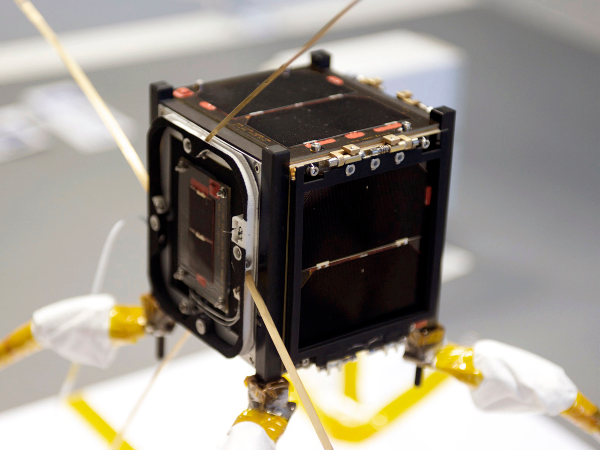
\includegraphics[width=0.5\textwidth]{Xatcobeo.pdf} %Xatcobeo.jpg
    \caption{Xatcobeo satellite photography (image from ESA-UVigo/INTA).}
    \label{fig:HumSat_Xatcobeo}
\end{figure}

Furthermore, there is a package to allow multiple figures to be defined within the same main figure, \emph{subcaption}.
With the code below, the author has the possibility to reference both the main figure (\autoref{fig:Trials_Setup}), or to reference each individual one (\autoref{fig:Trials_Setup_NetworkA} and \autoref{fig:Trials_Setup_NetworkB}).
%
\begin{figure}[!htb]
    \centering
    \begin{subfigure}[b]{0.48\textwidth}
        \centering
        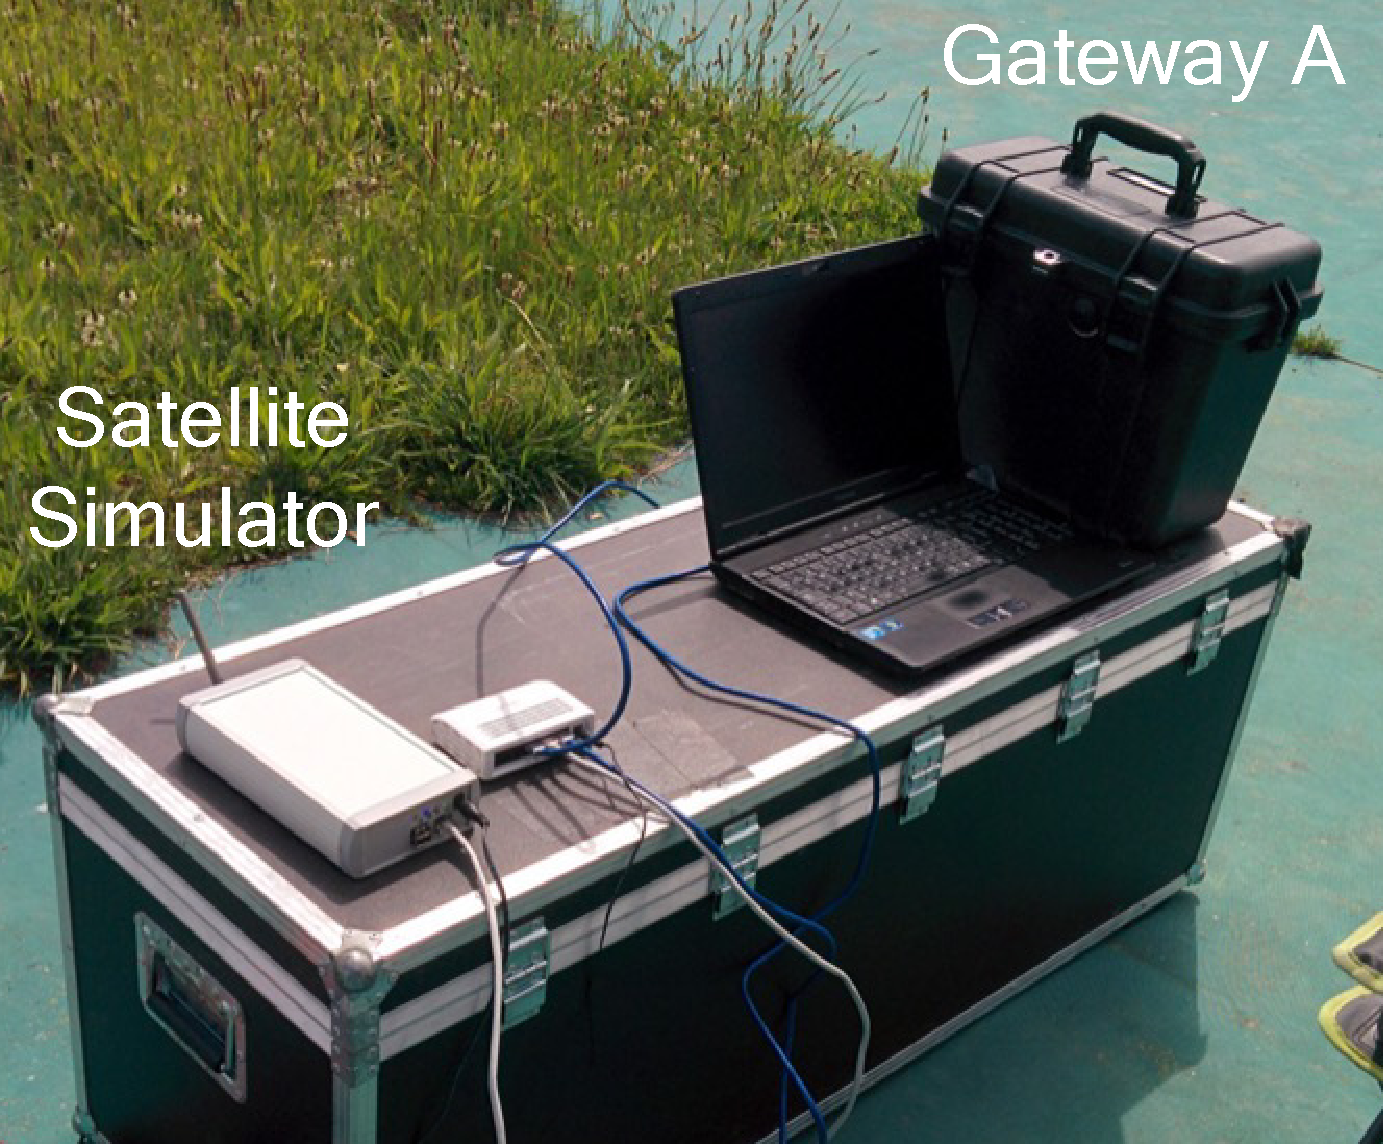
\includegraphics[width=0.97\textwidth]{NetworkA_FieldTry.pdf} %NetworkA_FieldTry.pdf
        \caption{Network A}
        \label{fig:Trials_Setup_NetworkA}
    \end{subfigure}
    \\ % To add a paragraph between figures.
    % Other options are possible, such as ~ or simply a blank line.
    \begin{subfigure}[b]{0.48\textwidth}
        \centering
        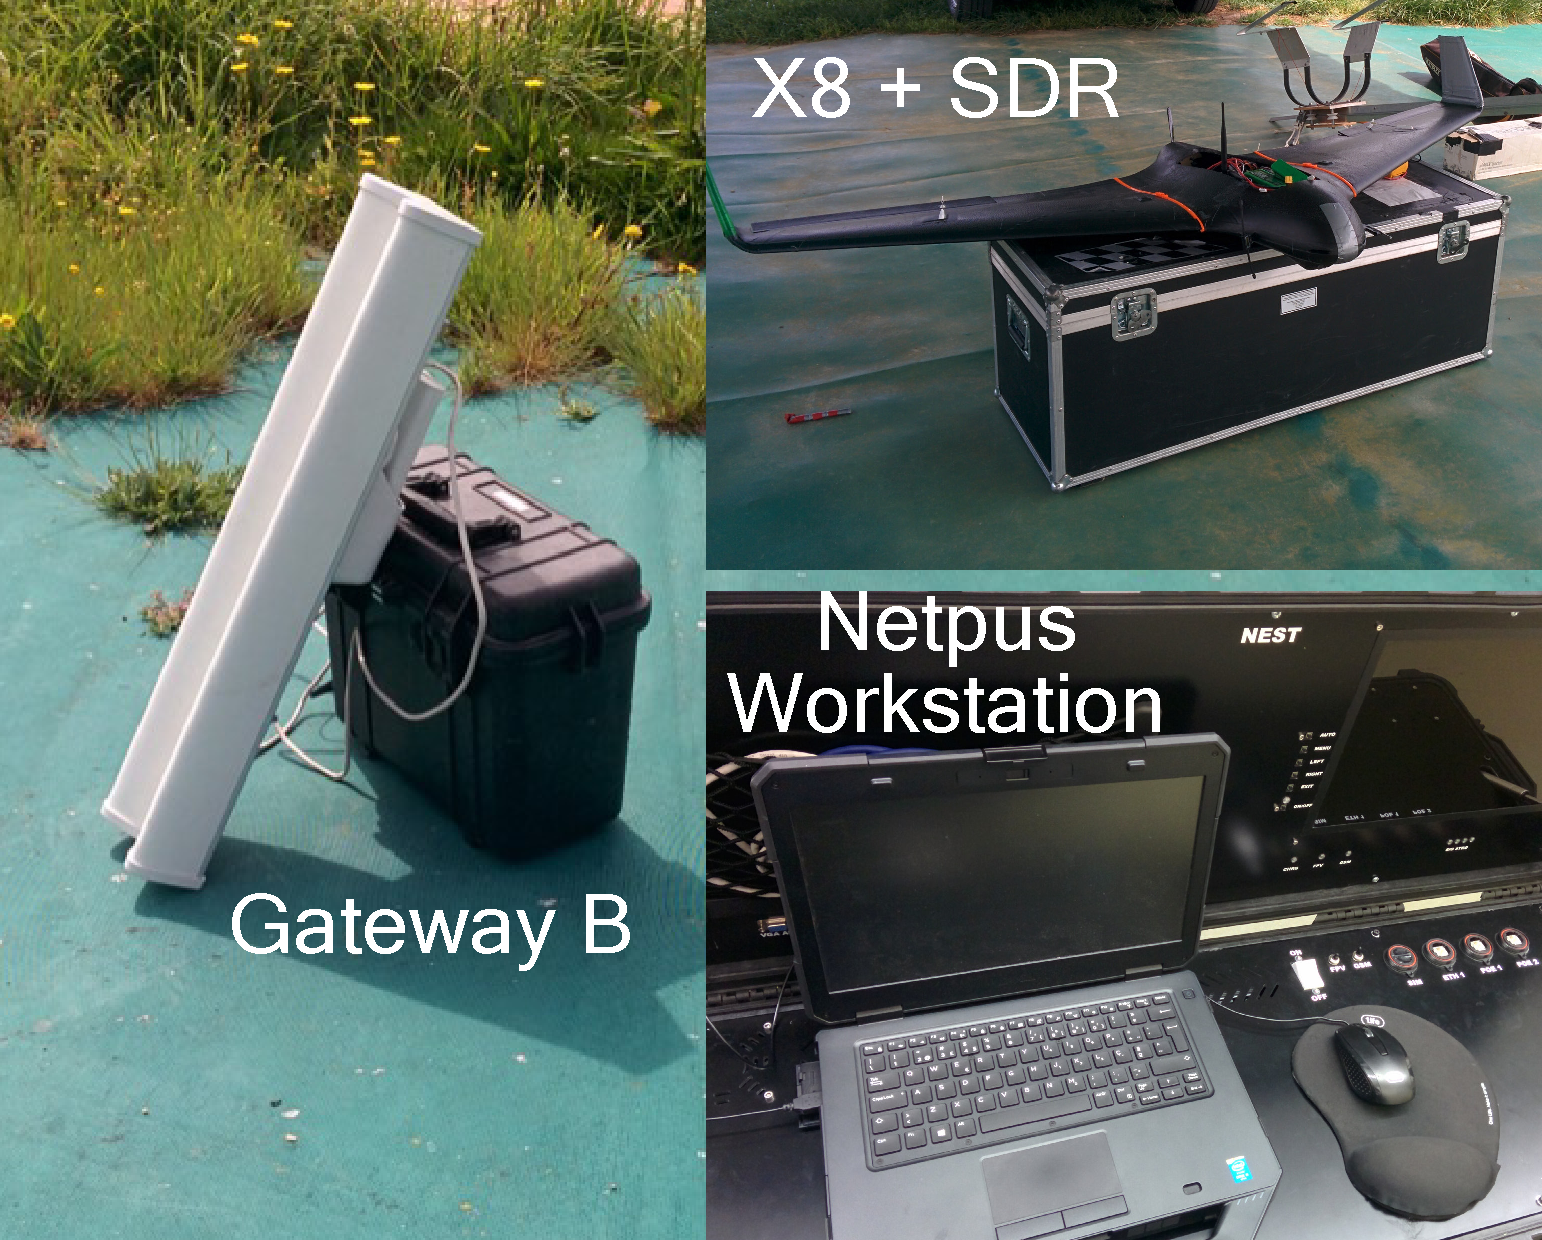
\includegraphics[width=1\textwidth]{NetworkB_FieldTry.pdf} %NetworkB_FieldTry.jpg
        \caption{Network B}
        \label{fig:Trials_Setup_NetworkB}
    \end{subfigure}
    \caption{Field trials operational setup.}
    \label{fig:Trials_Setup}
\end{figure}

For tables, besides the common \emph{booktabs} package, there is an extra one, \emph{threeparttable}, to create tables with footnotes in it.
The code for a table like this is shown below in~\autoref{tab:satcomm_comparison}
%
\begin{table}[!htb]
    %\scriptsize%\tiny
    \small
    %\setlength\tabcolsep{3.5pt}
    %\renewcommand{\arraystretch}{1.5}
    \centering
    \caption{Main characteristics of the satellite communication systems described (data from Refs.~\cite{Guerra2016}).}
    \label{tab:satcomm_comparison}
    \begin{threeparttable}
        \begin{tabular}{c >{\centering}m{1.8cm} c >{\centering}m{1.8cm} >{\centering}m{1.5cm} >{\centering}m{2cm} m{1.4cm}<{\centering}}
            \toprule
            System                      
            & Orbit Altitude [\si{km}]
            & Comm. Type    & Transmitting Power\tnote{\textdagger}\ \ [\si{W}]
            & Data rate\tnote{\textdagger}\ \ [\si{kbits/s}]   & Data Amount per Message\tnote{\textdagger}\ [\si{bytes}]
            & System of systems \\
            \midrule
            \multirow{2}[0]{*}{INMARSAT}
            & \multirow{2}[0]{\hsize}{\centering\num{35800} (GEO)}
            & Voice         & 100
            & 100                                           & --\tnote{$\ast$}
            & \multirow{2}[0]{*}{No} \\
            &
            & Data          & 9
            & --\tnote{$\ast$}                              & \num{6400}
            &  \\
            \multirow{2}[0]{*}{Iridium} 
            & \multirow{2}[0]{\hsize}{\centering780 (LEO)}
            & Voice         & 31
            & 134                                           & -
            & \multirow{2}[0]{*}{No} \\
            &
            & Data          & 1
            & 2.4                                           & 50
            &  \\
            Argos 
            & 800 (LEO)
            & Data          & 1
            & 4.8                                           & 31
            & No \\
            HumSat 
            & 600 (LEO)
            & Data          & 1
            & 1.2                                           & 32
            & Yes \\
            \bottomrule
        \end{tabular}
        \begin{tablenotes}
            \item[\textdagger] Values shown are top limits.
            \item[$\ast$] Information not available.
        \end{tablenotes}
    \end{threeparttable}
\end{table}

There is a package loaded to prevent figures from overstepping sections, \emph{placeins}.
This package besides being active for section, can also be modified to work with subsection.
Nevertheless, if the problem with a float going to the next subsection is localised, the command \emph{\textbackslash{}FloatBarrier} can be used after the float to prevent it from moving past that point.

Apart from these writing aspects, a package to handle and print a nomenclature was added, \emph{nomencl}.
To work with this package the author should add definitions as can be seen in file \textbf{01\_FrontMatter/Thesis\_Nomenclature}.



% ---------------------------------------------
% !TeX encoding = UTF-8
% !TeX spellcheck = en_GB
% !TeX root = ../ThesisTemplate_AndreGuerra.tex
%%%%%%%%%%%%%%%%%%% 11_Intro_Motivation.tex %%%%%%%%%%%%%%%%%%%%%%%%%%%%%%%
%
% PhD Thesis - Introduction - Motivation
% André Guerra
%
% 13/Dec/2017
%
%%%%%%%%%%%%%%%%%%%%%%%%%%%%%%%%%%%%%%%%%%%%%%%%%%%%%%%%%%%%%%%%%%%


% ---------------------------------------------
% ---------------------------------------------
\section{Motivation for small satellite oceanography}
\label{sec:Intro_Motivation}

{\small\textit{\lipsum[1-2]}}

% ---------------------------------------------
\subsection{The case for small satellite SAR}

{\small\textit{\lipsum[1-2]}}


% end of file 11_Intro_Motivation.tex
%%%%%%%%%%%%%%%%%%%%%%%%%%%%%%%%%%%%%%%%%%%%%%%%%%%%%%%%%%%%%%%%%%%

% ---------------------------------------------
% !TeX encoding = UTF-8
% !TeX spellcheck = en_GB
% !TeX root = ../Thesis_AndreGuerra.tex
%%%%%%%%%%%%%%%%%%% 12_Intro_CoordinatedObeservation.tex %%%%%%%%%%%%%%%%%%%%%%%%%%%%%%%
%
% PhD Thesis - Introduction - Coordinated Observation
% André Guerra
%
% 13/Dec/2017
%
%%%%%%%%%%%%%%%%%%%%%%%%%%%%%%%%%%%%%%%%%%%%%%%%%%%%%%%%%%%%%%%%%%%


% ---------------------------------------------
% ---------------------------------------------
\section{Coordinated observation with autonomous platforms}
\label{sec:Intro_CoordinatedObeservation}

{\small\textit{\lipsum[1-2]}}

% ---------------------------------------------
\subsection{Communication network}
\label{sec:Intro_CommNetwork}

{\small\textit{\lipsum[1-2]}}

% ---------------------------------------------
\subsection{The Portuguese case}
\label{sec:Intro_Portugal}

{\small\textit{\lipsum[1-2]}}


% end of file 12_Intro_CoordinatedObeservation.tex
%%%%%%%%%%%%%%%%%%%%%%%%%%%%%%%%%%%%%%%%%%%%%%%%%%%%%%%%%%%%%%%%%%%

% ---------------------------------------------
% !TeX encoding = UTF-8
% !TeX spellcheck = en_GB
% !TeX root = ../ThesisTemplate_AndreGuerra.tex
%%%%%%%%%%%%%%%%%%% 13_Intro_ThermalAnalysis.tex %%%%%%%%%%%%%%%%%%
%
% PhD Thesis - Introduction - Thermal Analysis
% André Guerra
%
% 18/Dec/2017
%
%%%%%%%%%%%%%%%%%%%%%%%%%%%%%%%%%%%%%%%%%%%%%%%%%%%%%%%%%%%%%%%%%%%


% ---------------------------------------------
% ---------------------------------------------
\section{Spacecraft design -- Thermal analysis and ensued accelerations}
\label{sec:Intro_Thermal}

{\small\textit{\lipsum[1-2]}}

% ---------------------------------------------
\subsection{Thermal radiation implications}
\label{sec:Intro_ThermalImplications}

{\small\textit{\lipsum[1-2]}}


% end of file 13_Intro_ThermalAnalysis.tex
%%%%%%%%%%%%%%%%%%%%%%%%%%%%%%%%%%%%%%%%%%%%%%%%%%%%%%%%%%%%%%%%%%%

% ---------------------------------------------
% ---------------------------------------------
\section{Objectives and outline}
\label{sec:Intro_OutlineObjectives}



% end of file 10_Intro.tex
%%%%%%%%%%%%%%%%%%%%%%%%%%%%%%%%%%%%%%%%%%%%%%%%%%%%%%%%%%%%%%%%%%%

%------------------------------------------------------------
% !TeX encoding = UTF-8
% !TeX spellcheck = en_GB
% !TeX root = ../Thesis_AndreGuerra.tex
%%%%%%%%%%%%%%%%%%% 20_SmallSat.tex %%%%%%%%%%%%%%%%%%%%%%%%%%%%%%%
%
% PhD Thesis - Small Satellites
% André Guerra
%
% 12/Dec/2017
%
%%%%%%%%%%%%%%%%%%%%%%%%%%%%%%%%%%%%%%%%%%%%%%%%%%%%%%%%%%%%%%%%%%%


% ---------------------------------------------
% ---------------------------------------------
\chapter{Small Satellites}
\label{chp:SmallSat}

% ---------------------------------------------
% ---------------------------------------------
\section{Brief history and classification}
\label{sec:SmallSat_HistoryClass}

\lipsum


% ---------------------------------------------
% ---------------------------------------------
\section{Features and components}
\label{sec:SmallSat_FeaturesComponents}

\lipsum

% ---------------------------------------------
\subsection{Structure and Mechanisms}
\label{subsec:Structures}

\lipsum

% ---------------------------------------------
\subsection{Propulsion System}
\label{subsec:Propulsion}

\lipsum

% ---------------------------------------------
\subsection{Attitude Determination \& Control System}
\label{subsec:ADCS}

\lipsum

% ---------------------------------------------
\subsection{Electric Power System}
\label{subsec:Power}

\lipsum

% ---------------------------------------------
\subsection{Thermal System}
\label{subsec:Thermal}

\lipsum

% ---------------------------------------------
\subsection{Command \& Data Handling}
\label{subsec:C_DH}

\lipsum

% ---------------------------------------------
\subsection{Communication Systems}
\label{subsec:Comm}

\lipsum

% ---------------------------------------------
\subsubsection{Regulating SmallSat Communication}
\label{subsec:Reg_Comm}

\lipsum


% ---------------------------------------------
% ---------------------------------------------
\section{Platform advantages and disadvantages}
\label{sec:SmallSat_AdvantDisadvanteges}

\lipsum


% end of file 20_SmallSat.tex
%%%%%%%%%%%%%%%%%%%%%%%%%%%%%%%%%%%%%%%%%%%%%%%%%%%%%%%%%%%%%%%%%%%

%------------------------------------------------------------
% !TeX encoding = UTF-8
% !TeX spellcheck = en_GB
% !TeX root = ../Thesis_AndreGuerra.tex
%%%%%%%%%%%%%%%%%%% 30_Ocean.tex %%%%%%%%%%%%%%%%%%%%%%%%%%%%%%%%%%
%
% PhD Thesis - Monitoring the Oceans with Small Satellites
% André Guerra
%
% 12/Dec/2017
%
%%%%%%%%%%%%%%%%%%%%%%%%%%%%%%%%%%%%%%%%%%%%%%%%%%%%%%%%%%%%%%%%%%%


% ---------------------------------------------
% ---------------------------------------------
\chapter{Monitoring the Oceans with Small Satellites}
\label{chp:Oceanography}


% ---------------------------------------------
% ---------------------------------------------
\section{Remote sensing oceanography}
\label{sec:Oceanography_RemoteSensing}

\lipsum


% ---------------------------------------------
% ---------------------------------------------
\section{Survey of ocean observing small satellites}
\label{sec:Oceanography_SmallSatSurvey}

\lipsum

% ---------------------------------------------
\subsection{Ocean Imaging}
\label{subsec:Ocean_Imaging}

\lipsum

% ---------------------------------------------
\subsection{Data Relay SmallSats}
\label{subsec:Data_Relay}

\lipsum

% ---------------------------------------------
\subsection{Tracking and AIS}
\label{subsec:AIS}

\lipsum

% ---------------------------------------------
\subsection{Constellations}
\label{subsec:Constellations}

\lipsum
    

% ---------------------------------------------
% ---------------------------------------------
\section{Sensors for oceanography}
\label{sec:Oceanography_Sensors}

\lipsum

% ---------------------------------------------
\subsection{Ocean colour}
\label{subsec:Ocean_colour}

\lipsum

% ---------------------------------------------
\subsection{Ocean altimetry}
\label{subsec:Ocean_altimetry}

\lipsum

% ---------------------------------------------
\subsection{Ocean surface winds}
\label{subsec:Ocean_winds}

\lipsum

% ---------------------------------------------
\subsection{Sea surface temperature}
\label{subsec:Ocean_temperature}

\lipsum

% ---------------------------------------------
\subsection{Ocean salinity}
\label{subsec:Ocean_salinity}

\lipsum

% ---------------------------------------------
\subsection{GNSS Reflectometry}
\label{subsec:GNSS_Reflectometry}

\lipsum

% ---------------------------------------------
\subsection{The case of (and for) SAR}
\label{subsec:SAR}

\lipsum


% end of file 30_Ocean.tex
%%%%%%%%%%%%%%%%%%%%%%%%%%%%%%%%%%%%%%%%%%%%%%%%%%%%%%%%%%%%%%%%%%%

%------------------------------------------------------------
% !TeX encoding = UTF-8
% !TeX spellcheck = en_GB
% !TeX root = ../Thesis_AndreGuerra.tex
%%%%%%%%%%%%%%%%%%% 40_NetworkOp.tex %%%%%%%%%%%%%%%%%%%%%%%%%%%%%%%%
%
% PhD Thesis - An Integrated Operation Scenario
% André Guerra
%
% 12/Dec/2017
%
%%%%%%%%%%%%%%%%%%%%%%%%%%%%%%%%%%%%%%%%%%%%%%%%%%%%%%%%%%%%%%%%%%%


% ---------------------------------------------
% ---------------------------------------------
\chapter{An Integrated Operation Scenario}
\label{chp:NetworkOp}


% ---------------------------------------------
% ---------------------------------------------
\section{Mission scenarios}
\label{sec:NetworkOp_Scenarios}

\lipsum


% ---------------------------------------------
% ---------------------------------------------
\section{LSTS network system}
\label{sec:NetworkOp_LSTS}

\lipsum

% ---------------------------------------------
\subsection{Software toolchain}

\lipsum

% ---------------------------------------------
\subsection{Autonomous vehicle system}

\lipsum


% ---------------------------------------------
% ---------------------------------------------
\section{Commercial communication systems}
\label{sec:NetworkOp_CommercialComms}

% ---------------------------------------------
\subsection{INMARSAT}
\label{sec:INMARSAT}

\lipsum

% ---------------------------------------------
\subsection{Iridium}
\label{sec:Iridium}

\lipsum

% ---------------------------------------------
\subsection{Argos}
\label{sec:Argos}

\lipsum


% ---------------------------------------------
% ---------------------------------------------
\section{The HumSat system}
\label{sec:NetworkOp_HumSat}

\lipsum

% ---------------------------------------------
\subsection{User Segment}
\label{sec:HumSat_User}

\lipsum

% ---------------------------------------------
\subsection{Space Segment}
\label{sec:HumSat_Space}

\lipsum
    

% ---------------------------------------------
% ---------------------------------------------
\section{System integration and test}
\label{sec:NetworkOp_Integration}

\lipsum

% ---------------------------------------------
\subsection{Software}
\label{sec:Integration_Software}

\lipsum

% ---------------------------------------------
\subsection{Hardware}
\label{sec:Integration_Hardware}

\lipsum

% ---------------------------------------------
\subsection{Tests and Results}
\label{sec:Integration_TestingWorkbench}

% ---------------------------------------------
\subsubsection{Workbench Tests}

\lipsum

% ---------------------------------------------
\subsubsection{Communication Dry-Run}

\lipsum

% ---------------------------------------------
\subsubsection{Field Trials}

\lipsum


% end of file 40_NetworkOp.tex
%%%%%%%%%%%%%%%%%%%%%%%%%%%%%%%%%%%%%%%%%%%%%%%%%%%%%%%%%%%%%%%%%%%

%------------------------------------------------------------
% !TeX encoding = UTF-8
% !TeX spellcheck = en_GB
% !TeX root = ../Thesis_AndreGuerra.tex
%%%%%%%%%%%%%%%%%%% 50_Thermal.tex %%%%%%%%%%%%%%%%%%%%%%%%%%%%%%%%
%
% PhD Thesis - Spacecraft and Small Satellite Thermal Analysis
% André Guerra
%
% 12/Dec/2017
%
%%%%%%%%%%%%%%%%%%%%%%%%%%%%%%%%%%%%%%%%%%%%%%%%%%%%%%%%%%%%%%%%%%%


% ---------------------------------------------
% ---------------------------------------------
\chapter{Spacecraft and Small Satellite Thermal Analysis}
\label{chp:Thermal}

    
% ---------------------------------------------
\section{The thermal subsystem – Tasks and objectives}
\label{sec:Thermal_Subsystem}

 {\small\textit{\lipsum[1-2]}}




% ---------------------------------------------
\section{Space thermal environment}
\label{sec:Thermal_Environment}

 {\small\textit{\lipsum[1-2]}}



% ---------------------------------------------
\section{Thermal control technology}
\label{sec:Thermal_Technology}

 {\small\textit{\lipsum[1-2]}}




% ---------------------------------------------
\section{Computational analysis methods}
\label{sec:Thermal_Methods}

 {\small\textit{\lipsum[1-2]}}



% ---------------------------------------------
% ---------------------------------------------
\section{A practical case}
\label{sec:Thermal_Pratical}

 {\small\textit{\lipsum[1-2]}}

% ---------------------------------------------
\subsection{Geometric Model}
\label{sec:GeometricModel}

 {\small\textit{\lipsum[1-2]}}

% ---------------------------------------------
\subsection{Analysis Cases and Assumptions}
\label{sec:Analysis}

 {\small\textit{\lipsum[1-2]}}

% ---------------------------------------------
\subsubsection{Global Assumptions}
\label{subsec:Assumptions}

 {\small\textit{\lipsum[1-2]}}

% ---------------------------------------------
\subsubsection{Operational Conditions}
\label{subsec:OpConditions}

 {\small\textit{\lipsum[1-2]}}

% ---------------------------------------------
\subsection{Results and Discussion}
\label{sec:Results}

 {\small\textit{\lipsum[1-2]}}

% ---------------------------------------------
\subsubsection{Amplifier Off}
\label{sec:AmpOff}

 {\small\textit{\lipsum[1-2]}}

% ---------------------------------------------
\subsubsection{Amplifier On}
\label{sec:AmpOn}

 {\small\textit{\lipsum[1-2]}}

% ---------------------------------------------
\subsubsection{Temperature Distribution -- Amplifier On}
\label{sec:TempDist_AmpOn}

 {\small\textit{\lipsum[1-2]}}


% ---------------------------------------------
% ---------------------------------------------
\section{Another approach to thermal analysis and induced accelerations}
\label{sec:Thermal_Accelerations}

 {\small\textit{\lipsum[1-2]}}

% ---------------------------------------------
\subsection{Pointlike Source Method}
\label{sec:Source_method}

 {\small\textit{\lipsum[1-2]}}

% ---------------------------------------------
\subsubsection{Motivation}
\label{subsec:Source_method_motivation}

 {\small\textit{\lipsum[1-2]}}

% ---------------------------------------------
\subsubsection{Radiative Momentum Transfer}
\label{subsec:RadMomTransf}

 {\small\textit{\lipsum[1-2]}}

% ---------------------------------------------
\subsubsection{Reflection Modelling -- Phong Shading}
\label{subsec:Phong}

 {\small\textit{\lipsum[1-2]}}

% ---------------------------------------------
\subsubsection{Computation of Reflection}
\label{subsec:reflection_computation}

 {\small\textit{\lipsum[1-2]}}

% ---------------------------------------------
\subsection{New Horizons Model}
\label{sec:NH_Model}

 {\small\textit{\lipsum[1-2]}}

% ---------------------------------------------
\subsubsection{Physical Setup}

 {\small\textit{\lipsum[1-2]}}

% ---------------------------------------------
\subsubsection{Power Supply}
\label{subsec:Power_Supply}

 {\small\textit{\lipsum[1-2]}}

% ---------------------------------------------
\subsubsection{Thermal Emissions Modelling}
\label{sec:Initial_Study}

 {\small\textit{\lipsum[1-2]}}

% ---------------------------------------------
\subsection{Results and Discussion}
\label{sec:Results_Discussion}

 {\small\textit{\lipsum[1-2]}}

% ---------------------------------------------
\subsubsection{Baseline Scenarios}
\label{subsec:Scenarios}

 {\small\textit{\lipsum[1-2]}}

% ---------------------------------------------
\subsubsection{Parametric Study}
\label{subsec:parametric_study}

 {\small\textit{\lipsum[1-2]}}

% ---------------------------------------------
\subsubsection{Results of the Thermal Effects on Attitude}
\label{sec:attitude_results}

 {\small\textit{\lipsum[1-2]}}



% end of file 50_Thermal.tex
%%%%%%%%%%%%%%%%%%%%%%%%%%%%%%%%%%%%%%%%%%%%%%%%%%%%%%%%%%%%%%%%%%%

%------------------------------------------------------------
% !TeX encoding = UTF-8
% !TeX spellcheck = en_GB
% !TeX root = ../ThesisTemplate_AndreGuerra.tex
%%%%%%%%%%%%%%%%%%% 60_Conclusion.tex %%%%%%%%%%%%%%%%%%%%%%%%%%%%%
%
% PhD Thesis - Conclusions
% André Guerra
%
% 12/Dec/2017
%
%%%%%%%%%%%%%%%%%%%%%%%%%%%%%%%%%%%%%%%%%%%%%%%%%%%%%%%%%%%%%%%%%%%


% ---------------------------------------------
% ---------------------------------------------
\chapter{Conclusions}
\label{chp:Conclusions}

{\small\textit{\lipsum[1-2]}}




% end of file 60_Conclusion.tex
%%%%%%%%%%%%%%%%%%%%%%%%%%%%%%%%%%%%%%%%%%%%%%%%%%%%%%%%%%%%%%%%%%%


%------------------------------------------------------------
%% Bibliography -------------------------------------------%%
\renewcommand{\bibname}{References}
\addcontentsline{toc}{chapter}{References}
%%\bibliographystyle{unsrtnat}
\bibliographystyle{elsarticle-num}
%%\bibliographystyle{0_Layout/phd_style}
%\begin{small}
\bibliography{%
    70_Bibliography/Introduction_BIB,%
    70_Bibliography/SmallSat_BIB,%
    70_Bibliography/Ocean_BIB,%
    70_Bibliography/NetworkOp_BIB,%
    70_Bibliography/Thermal_BIB,%
    70_Bibliography/Appendix_BIB}
%\end{small}

%------------------------------------------------------------
%% Appendix -----------------------------------------------%%
\appendix
%%%\begin{appendices}
%%%\end{appendices}

%------------------------------------------------------------
% !TeX encoding = UTF-8
% !TeX spellcheck = en_GB
% !TeX root = ../Thesis_AndreGuerra.tex
%%%%%%%%%%%%%%%%%%% 81_Appendices_SAR.tex %%%%%%%%%%%%%%%%%%%%%%%%%%%%%
%
% PhD Thesis - Appendices - SAR
% André Guerra
%
% 16/Dec/2017
%
%%%%%%%%%%%%%%%%%%%%%%%%%%%%%%%%%%%%%%%%%%%%%%%%%%%%%%%%%%%%%%%%%%%


% ---------------------------------------------
% ---------------------------------------------
\chapter{SAR Principles}
\label{chp:SAR_Principles}

{\small\textit{\lipsum[1-2]}}


% end of file 81_Appendices_SAR.tex
%%%%%%%%%%%%%%%%%%%%%%%%%%%%%%%%%%%%%%%%%%%%%%%%%%%%%%%%%%%%%%%%%%%

% !TeX encoding = UTF-8
% !TeX spellcheck = en_GB
% !TeX root = ../Thesis_AndreGuerra.tex
%%%%%%%%%%%%%%%%%%% 82_Appendices_ThermalAttitude.tex %%%%%%%%%%%%%%%%%%%%%%%%%%%%%
%
% PhD Thesis - Appendices - Thermal Attitude Effects
% André Guerra
%
% 18/Dec/2017
%
%%%%%%%%%%%%%%%%%%%%%%%%%%%%%%%%%%%%%%%%%%%%%%%%%%%%%%%%%%%%%%%%%%%


% ---------------------------------------------
% ---------------------------------------------
\chapter{Modelling the Thermal Effects on the Attitude of the Spacecraft}
\label{chp:Thermal_attitude}



% ---------------------------------------------
\section{Thermal Moment Relative to the Centre of Mass}
\label{subsec:thermal_moment}

 {\small\textit{\lipsum[1-2]}}



% ---------------------------------------------
\section{Rotation Dynamics Induced by Thermal Effects}
\label{subsec:thermal_rotation}

 {\small\textit{\lipsum[1-2]}}



% ---------------------------------------------

\subsection{Spin Stabilised Case}
\label{subsec:spinsatibised_case}

 {\small\textit{\lipsum[1-2]}}



% ---------------------------------------------
\subsection{Three-Axis Mode Case}
\label{subsec:threeaxis_case}

 {\small\textit{\lipsum[1-2]}}





% end of file 82_Appendices_ThermalAttitude.tex
%%%%%%%%%%%%%%%%%%%%%%%%%%%%%%%%%%%%%%%%%%%%%%%%%%%%%%%%%%%%%%%%%%%


% ----------------------------------------------------------------------
\end{document}
% end of file Thesis_AndreGuerra.tex
%%%%%%%%%%%%%%%%%%%%%%%%%%%%%%%%%%%%%%%%%%%%%%%%%%%%%%%%%%%%%%%%%%%